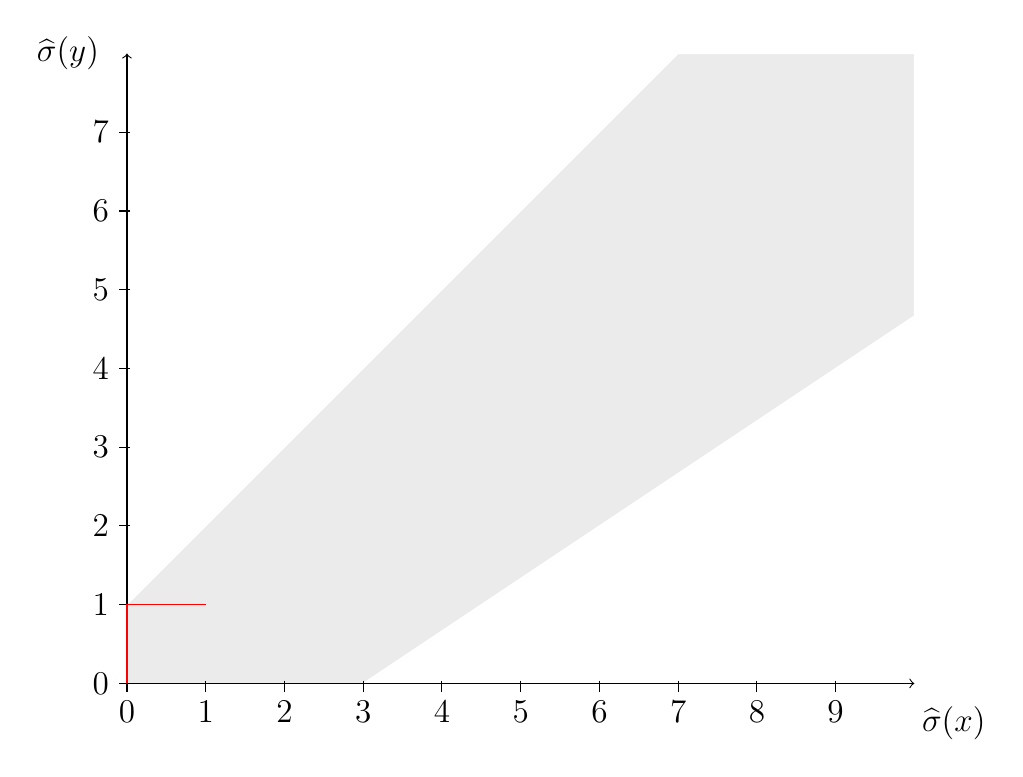
\begin{tikzpicture}[only marks]

    % Pintamos el fondo del poliedro
    \draw[color=white, fill=black!8] (0,1) -- (7,8) -- (10,8) -- (10,14/3) -- (3,0) -- (0,0);
        
    % Dibujamos los ejes
    \draw[->] (0,0) -- coordinate (x axis mid) (10,0);
    \draw[->] (0,0) -- coordinate (y axis mid)(0,8);

    % Marcamos los ejes
    \foreach \x in {0,1,2,3,4,5,6,7,8,9}
        \draw [](\x cm,1pt) -- (\x cm,-3pt)
            node[anchor=north] {\large $\x$};
    \foreach \y in {0,1,2,3,4,5,6,7}
        \draw (1pt,\y cm) -- (-3pt,\y cm) node[anchor=east] {\large $\y$};

    % Nombramos los ejes
    \node[] (sigmax) at (10.5,-.5) {\large $\widehat\sigma(x)$};                    
    \node[] (sigmay) at (-.75,8) {\large $\widehat\sigma(y)$};                                   
        
% Caminata roja
\path[draw, color=red] (0,0) -- (0,1) -- (1,1);
      
\end{tikzpicture}
